\documentclass[11pt,twoside]{article}

\usepackage{amsmath}
\usepackage{graphicx,epsfig}
\usepackage{graphicx}
\usepackage{amsmath,amssymb,amsbsy,bm}
%\usepackage[framed]{mcode}

\newlength{\toppush}
\setlength{\toppush}{2\headheight}
\addtolength{\toppush}{\headsep}

\renewcommand{\bottomfraction}{0.95}

\newcommand{\htitle}[3]{\begin{center}
\vspace*{-\toppush}
{\large MASSACHUSETTS INSTITUTE OF TECHNOLOGY}\\
{\small Department of Electrical Engineering and Computer Science}\\
\vspace*{1ex}{\Large #2}\end{center}
\noindent
\newline\parbox{6.5in}
{Fall 2013\hfill Issued : #1 \newline
 Problem Set 4 \hfill Due : #3\newline
%\profs \hfill %Handout #1\vspace*{-.5ex}\newline
%\mbox{}\hrulefill\mbox{}
}}

\newcommand{\mcO}{\mathcal{O}}
\newcommand{\handout}[3]{\thispagestyle{empty}
\pagestyle{myheadings}\htitle{#1}{#2}{#3}}

\setlength{\oddsidemargin}{0pt}
\setlength{\evensidemargin}{0pt}
\setlength{\textwidth}{6.5in}
\setlength{\topmargin}{0in}
\setlength{\textheight}{8.5in}


\newcommand{\pp}[2]{\frac{\partial #1}{\partial #2}}%
\newcommand{\ppp}[2]{\frac{\partial^2 #1}{\partial #2^2}}%
\newcommand{\dd}[2]{\frac{d #1}{d #2}}%
\newcommand{\ddd}[2]{\frac{d^2 #1}{d #2^2}}%
\newcommand{\matend}{\end{array}\right]}
\newcommand{\matc}{\left[\begin{array}{c}}
\newcommand{\matcc}{\left[\begin{array}{cc}}
\newcommand{\bb}{\mathbf{b}}
\newcommand{\bx}{\mathbf{x}}
\newcommand{\bA}{\mathbf{A}}
\newcommand{\DD}[2]{\frac{D #1}{D #2}}%
\newcommand{\Uvec}{\mathbf{U}}
\newcommand{\uvec}{\mathbf{u}}
\newcommand{\tauvec}{\bm{\tau}}
\newcommand{\omegavec}{\bm{\omega}}


\renewcommand{\Re}{\mathrm{Re}}


\begin{document}


\handout{Oct 1, 2013}{6.301 Solid State Circuits}{Oct 8, 2013}
\setlength{\parindent}{0pt}

\newcommand{\solution}{
 \medskip
 {\bf Solution:}
}

\hrulefill

\flushleft

\subsection*{Problem 1: Building Blocks}
The AC schematics for four amplifiers are shown below.
For each of the amplifiers, find the midband voltage gain and the -3dB frequency using the open-circuit time-constant method.
Assume $/beta=200$, $I_C=2.5mA$, $c_\pi=50pF$, and $c_\mu=2pf$.
Neglect $r_b$ and $r_o$.
\begin{enumerate}
	\item[\bf(a)] Common Emitter:
\begin{center}
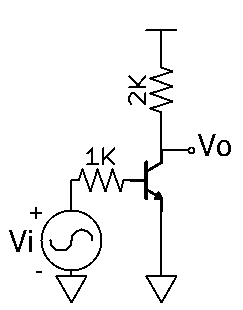
\includegraphics[width=0.25\textwidth]{ce.png}
\end{center}
	\item[\bf(b)] Emitter Follower:
\begin{center}
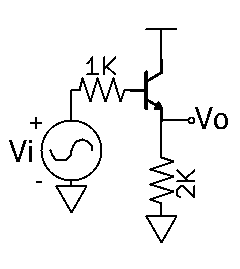
\includegraphics[width=0.25\textwidth]{ef.png}
\end{center}
\clearpage
	\item[\bf(c)] Common Base:
\begin{center}
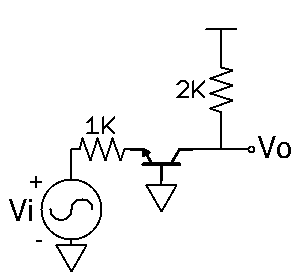
\includegraphics[width=0.3\textwidth]{cb.png}
\end{center}
	\item[\bf(d)] Common Emitter with Emitter Degeneration:
\begin{center}
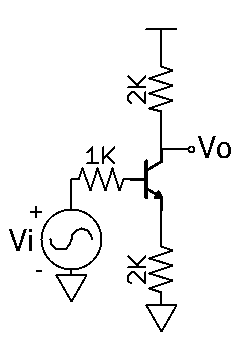
\includegraphics[width=0.25\textwidth]{ceed.png}
\end{center}
\end{enumerate}

\subsection*{Problem 2: Two-transistor OCTs}
For the following CB-CE amplifier, assume $V_{BE}=0.6v$, $\beta=200$, $c_\pi=20pF$, and $c_\mu=2pF$.
Neglect $r_b$ and $r_o$.

\begin{enumerate}
	\item[\bf(a)] Calculate the midband voltage gain.
	\item[\bf(b)] Find the -3dB frequency of the amplifier using the OCT method.
\end{enumerate}

\subsection*{Problem 3: Emitter Coupled Pairs}
For the two amplifiers shown below, find the midband voltage gain and the -3dB frequency.
Why does one have more bandwidth than the other? \\
You may assume $V_{BE}=0.6v$, $\beta=400$, $c_\pi=40pF$, $c_\mu=4pF$, and neglect $r_b$ and $r_o$.

\begin{enumerate}
	\item[\bf(a)] Single-ended Differential Pair
	\item[\bf(b)] EF-CB
\end{enumerate}

\subsection*{Problem 4: Buffered Diff Pair}


\clearpage
\end{document}
